\section{Dataset Description}
\label{sec:dataset_description}
In Chapter \ref{chapter:research_plan}, we have outlined our primary research focus, which revolves around the field of Vision-Based Multi-Task Imitation Learning. Specifically, we are directing our attention to Video-Conditioned methods, with reference to seminal works such as \cite{mandi2022towards_more_generalizable_one_shot} and \cite{dasari2021transformers_one_shot}, which have been chosen as our initial reference points due to their promising outcomes as presented in Table \ref{table:mosaic}.
Within the realm of Vision-Based Multi-Task Imitation Learning, we aim to establish a robust baseline for tasks that encompass a blend of highly multimodal behaviors and intricate fine-grained manipulations. To achieve this, we have commenced our investigations by narrowing our focus to two specific tasks: \textit{``Pick-and-Place"} and \textit{``Nut-Assembly"} both of which are proposed among the seven tasks in \cite{mandi2022towards_more_generalizable_one_shot}.
The information in Table \ref{table:reference_dataset_cardinality} provides a summary of the dataset's cardinality, including the number of variations for each task and the number of trajectories. These statistics align closely with the parameters outlined in \cite{mandi2022towards_more_generalizable_one_shot}.
\begin{table}[htb]
    \centering
    \caption{Reference dataset's cardinality}
    \label{table:reference_dataset_cardinality}
    \begin{tblr}{
        width = \linewidth,
        colspec = {Q[192]Q[165]Q[387]Q[190]},
        cells = {c},
        hlines,
        hline{1,4} = {-}{0.08em},
            }
                              & \textbf{\#Variations} & \textbf{\#Trajectories per variations} & \textbf{\#Trajectories} \\
        \textit{Pick-Place}   & 16                    & 100                                    & 1600                    \\
        \textit{Nut-Assembly} & 9                     & 100                                    & 900
    \end{tblr}
\end{table}
Moreover, Figure \ref{fig:example_of_variations_for_pick_place} and Figure \ref{fig:examples_of_variations_for_nut_assembly} depicts some variation examples for each task.
As it can be noted the designed scenarios show some degree of difficulties from a \textit{perception point of view}, that can be summirized as follow:
\begin{itemize}
    \item The scene is composed of objects, that differ only from high-level features such as the color. This poses a challenge for Deep Convolutional Based methods, as these techniques typically excel at learning and distinguishing \textit{\textbf{lower-level features}}, making the recognition of objects based solely on attributes like color a demanding task.
    \item The object that in a given variation is a distractor in another variation is the target object. This poses a significant challenge because the method cannot learn a pre-established pattern where a specific category of objects consistently assumes the role of the target while another category consistently acts as a distractor. Consequently, the demonstration video and its role in conditioning the policy become pivotal factors in addressing this challenge.
\end{itemize}
As discussed in Section \ref{sec:experiment_results}, these factors play a pivotal role and can significantly impact the performance of the methods employed.
\begin{figure}[hbt!]
    \centering
    \begin{subfigure}{0.2\textwidth}
        \centering
        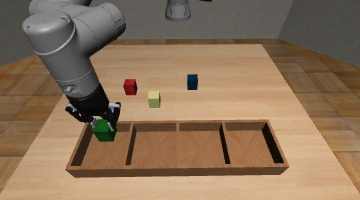
\includegraphics[width=\textwidth]{Figures/images/pick_place/task_1.png}
        \caption{First variation, green box into first bin}
        \label{fig:first_variation}
    \end{subfigure}
    \hfill
    \begin{subfigure}{0.2\textwidth}
        \centering
        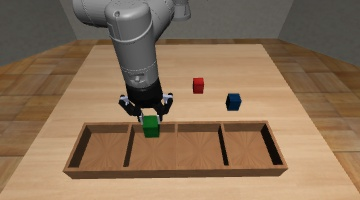
\includegraphics[width=\textwidth]{Figures/images/pick_place/task_2.png}
        \caption{Second variation, green box into second bin}
        \label{fig:second_variation}
    \end{subfigure}
    \hfill
    \begin{subfigure}{0.2\textwidth}
        \centering
        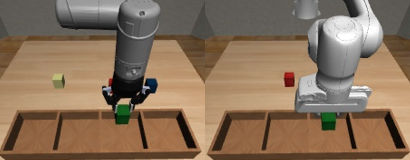
\includegraphics[width=\textwidth]{Figures/images/pick_place/task_3.png}
        \caption{Third variation, green box into third bin}
        \label{fig:third_variation}
    \end{subfigure}
    \hfill
    \begin{subfigure}{0.2\textwidth}
        \centering
        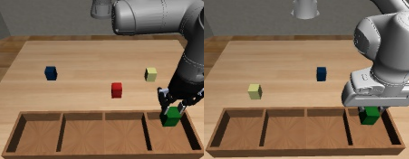
\includegraphics[width=\textwidth]{Figures/images/pick_place/task_4.png}
        \caption{Fourth variation, green box into fourth bin}
        \label{fig:fourth_variation}
    \end{subfigure}
    \caption{Example of variations for the Pick and Place task. The same set of variations is repeated for each block}
    \label{fig:example_of_variations_for_pick_place}
\end{figure}

\begin{figure}[hbt!]
    \centering
    \begin{subfigure}{0.2\textwidth}
        \centering
        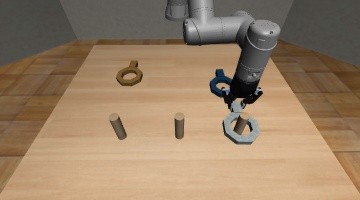
\includegraphics[width=\textwidth]{Figures/images/nut_assembly/task_1.png}
        \caption{First variation, assembly gray nut with right peg}
        \label{fig:first_variation_nut}
    \end{subfigure}
    \hspace{30px}
    \begin{subfigure}{0.2\textwidth}
        \centering
        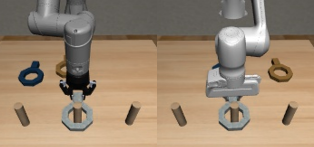
\includegraphics[width=\textwidth]{Figures/images/nut_assembly/task_2.png}
        \caption{Second variation, assembly gray nut with middle peg}
        \label{fig:second_variation_nut}
    \end{subfigure}
    \hspace{30px}
    \begin{subfigure}{0.2\textwidth}
        \centering
        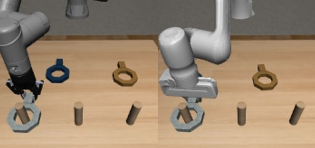
\includegraphics[width=\textwidth]{Figures/images/nut_assembly/task_3.png}
        \caption{Third variation, assembly gray nut with left peg}
        \label{fig:third_variation_nut}
    \end{subfigure}
    \caption{Example of variations for the Nut-Assembly. The same set of variations is repeated for each nut}
    \label{fig:examples_of_variations_for_nut_assembly}
\end{figure}
Another critical consideration pertaining to the dataset concerns the distribution of actions. This aspect is exemplified in Figure \ref{fig:dataset_distribution}, which illustrates the trajectory distribution along the x-y-z axes for the initial variation of both Pick-and-Place and Nut-Assembly tasks. It is evident that, for a given variation, the target object exhibits varying starting positions. This characteristic adds a layer of complexity to the learning task at hand, as the model must be adept at identifying the target object within the image, even when its initial pose differs across different instances. The significance of this challenge is magnified since it is a pervasive issue across all subsequent variations of both Pick-and-Place and Nut-Assembly tasks. Consequently, the need for the model to generalize across different starting positions of the target object poses a substantial obstacle in achieving robust and reliable performance in this dataset.
\begin{figure}[htb]
    \centering
    \begin{subfigure}[b]{0.9\textwidth}
        \centering
        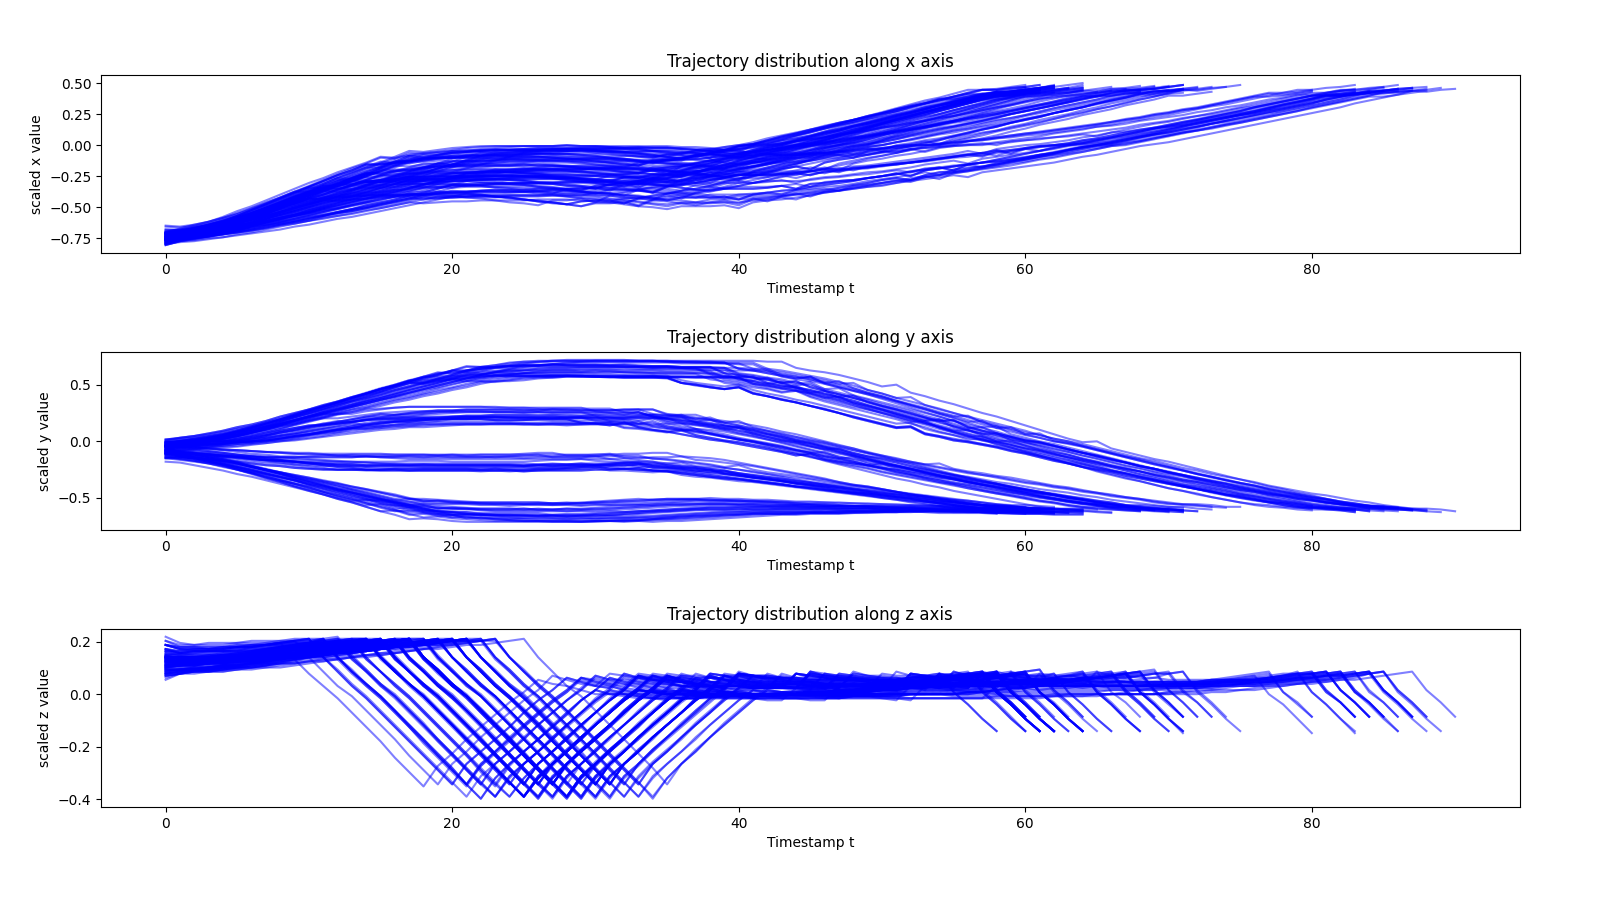
\includegraphics[width=\textwidth]{Figures/images/dataset_distribution/pick_place_variation_0.png}
        \caption{Trajectory distribution along the x-y-z axes for the first Pick-Place variation}
        \label{fig:pick_place_first_variation}
    \end{subfigure}
    \hfil
    \begin{subfigure}[b]{0.9\textwidth}
        \centering
        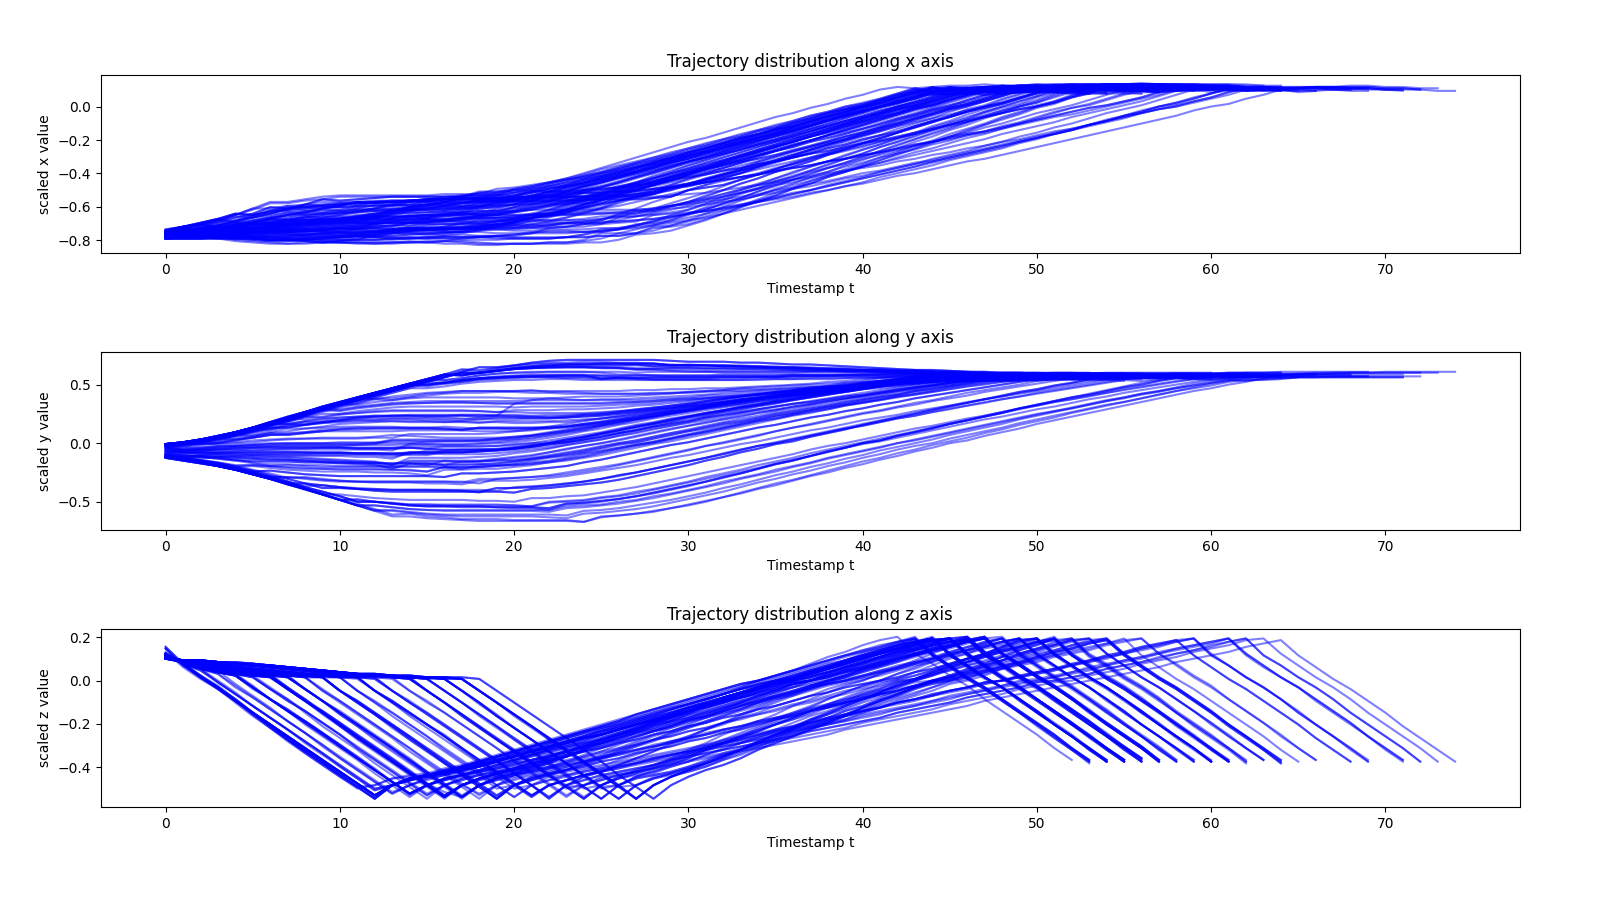
\includegraphics[width=\textwidth]{Figures/images/dataset_distribution/nut_assembly_variation_0.png}
        \caption{Trajectory distribution along the x-y-z axes for the first Nut-Assembly variation}
        \label{fig:nut_assembly_first_variation}
    \end{subfigure}
    \caption{Trajectory Distribution along the x-y-z axes for the first variation of Pick-Place (\ref{fig:pick_place_first_variation}) and Nut-Assembly (\ref{fig:nut_assembly_first_variation}) task}
    \label{fig:dataset_distribution}
\end{figure}

